\documentclass[titlepage]{jsreport}

\usepackage[dvipdfmx]{graphicx}
\usepackage{listings}
\usepackage{url}
\usepackage{bm}
\usepackage{cite}

% ソースコードを挿入するための設定
\lstset{
 	language = Python,
     frame = tbrl
}

\title{ガウス過程回帰を用いた効率的な状態方程式推定及び相図探索}
\author{慶應義塾大学理工学部物理情報工学科\\
指導教員 渡辺宙志\\
学籍番号 61713173\\
内藤翔太}
\date{2020年MM月DD日}

\begin{document}

\maketitle

\tableofcontents

\chapter{はじめに} \label{chap:introduction}

\section{研究の背景} \label{intro-background}
様々な実存気体の状態方程式の推定や、相図の作成は物性物理の分野において非常に重要な役割を果たす。
粒子系の相図、特に温度-数密度をパラメタにとった相図作成には、圧力の温度$T$、数密度$\rho$依存性をあらゆる温度$T$、数密度$\rho$で測定する必要が生じるが、
これは、圧力$P$を温度$T$、数密度$\rho$に関する項で書き下す状態方程式の微分不連続の線を探すことと同義とみなせる。

実存気体の状態方程式を再現しようとする試みは、1901年にHeikeが提唱したビリアル展開\cite{virial-Heike}、
1940年にManson、George、Rubinが提唱したBenedict-Webb-Rubin\,(BWR)方程式\cite{BWR-equation:original}、1973年にJacobsen、Stewartが提唱したmodified-Benedict-Webb-Rubin\,(mBWR)方程式\cite{m-BWR-equation}
を応用することにより、多くの研究者により行われてきた\cite{MCCARTY1974276,BWR-equation:13,BWR-equation:25}。
これらの多くの研究者の努力により、実存気体を広い範囲で概ね再現する有効な状態方程式を構築することに成功したが、
その精度は十分とは言えず、項の個数は際限なく増え、項自体の物理的意味も不明瞭であった。

相図の作成は、実用性が高い反面、手間とコストがかかる作業である。
従来は、この手間とコストを削減するためにグリッド探索\cite{grid1,grid2}を用いていたが、事前にグリッド上に一様に配置された状態点を実験し評価するグリッド探索は、
以前の実験からの情報を抽出できないため非効率であった。
そこで、近年では、不確実性サンプリング\cite{uncertainty-sampling1,uncertainty-sampling2}やガウス過程回帰\cite{gaussian-phase}といった高度なサンプリングアルゴリズムを実装することにより、
手間とコストを削減することに成功している。
しかし、これらの研究は状態点の相が全て判別されている前提で、それを知らない機械がその中から必要な状態点を取得し、状態点の相を形式的に効率的に特定しているに過ぎない。


\section{研究の目的} \label{intro-purpose}
様々な実存気体の状態方程式は\ref{intro-background}節で述べたように、ビリアル展開・BWR方程式・m-BWR方程式を応用し、項の個数を増やすことによって広範囲である程度有効なものを構築することに成功したが、
項の個数は際限なく増え、その物理的意味も不明瞭であった。
そこで、ビリアル展開・BWR方程式・m-BWR方程式を用いて状態方程式の項の係数を決定するのではなく、
機械学習により、より多くの項の候補から状態方程式を推定することが1つ目の目的である。
また相図の作成は、\ref{intro-background}節で述べたように、様々な高度なサンプリングアルゴリズムにより効率的に行われてきたが、
これらの研究は予め状態点の相が全て判別されている前提で、それを知らない機械がその中から必要な状態点を取得し、状態点の相を形式的に効率的に特定しているに過ぎない。
つまり、この手法は状態点の相が分からない未知の系に適用する際、状態点の相を効率的に特定する手法とは言えない。
そこで、状態点の相が分からない未知の系に対しても相図作成が自動でできるような手法、すなわち機械が次の状態点を選択し、
その状態点における相を自動的に特定していくような手法を構築するのが2つ目の目的である。
本研究では上記の2点の目的を受け、状態方程式が比較的容易に書け、状態点の相の判別が容易であるWeeks-Chandler-Andersen\,(WCA)ポテンシャル粒子系を採用する。
WCAポテンシャル粒子系では、温度一定のまま数密度を高くしていくと、ある数密度で流体相から固体相への相転移を起こす。
\ref{intro-background}節でも述べたように、相転移近傍では、圧力の振る舞いが大きく変化するので、圧力$P$と数密度$\rho$の関係を調べることで状態方程式の推定を行いつつ、相転移の存在を確認し、WCAポテンシャル粒子系における相図も作成することが出来る。

本研究においては、上記の2点の目的の前身として、WCAポテンシャル粒子系における圧力$P$を数密度$\rho$に関する低次の多項式で近似することにより状態方程式を推定できることを確認した上で、
ガウス過程回帰を適用することにより、状態方程式を効率的に推定しつつ、相図を効率的に作成することを目的とする。


\section{本論文の構成} \label{intro-constitution}
本研究では、WCAポテンシャル粒子系における圧力$P$を数密度$\rho$に関する低次の多項式で近似することにより状態方程式を推定できることを確認した上で、
ガウス過程回帰を適用することにより、状態方程式を効率的に推定しつつ、相図を効率的に作成することを目的とする。

第\ref{chap:introduction}章では、実存気体の状態方程式の推定及び相図作成に用いられている手法を示した。
第\ref{chap:method}章では、WCAポテンシャル粒子系における状態方程式の推定と相図の作成を効率的に行う手法を示す。
第\ref{chap:results}章では、第\ref{chap:method}章で提案した手法の精度の確認を行う。
第\ref{chap:summary}章では本研究で得られた知見を総括し、結論と今後の展望について述べる。


\chapter{手法} \label{chap:method}
\ref{method-sec:WCA-press}節では、WCAポテンシャル粒子系において各数密度$\rho$における圧力$P$を定義し、圧力$P$と数密度$\rho$の関係を調べる。
\ref{method-sec:WCA-equation}節では、\ref{results-sec:WCA-press}節で得た圧力$P$と数密度$\rho$の関係から、WCAポテンシャル粒子系における状態方程式の推定を行う。
\ref{method-sec:Gauss}節では、\ref{results-sec:WCA-press}節で得た圧力$P$と数密度$\rho$の関係にガウス過程回帰を適用し、
WCAポテンシャル粒子系における状態方程式を効率的に推定しつつ、相図を効率的に作成する。


\section{WCAポテンシャル粒子系における圧力測定}\label{method-sec:WCA-press}
\ref{method-sec:WCA-press}節ではWCAポテンシャル粒子系において各数密度$\rho$における圧力$P$を定義し、圧力$P$と数密度$\rho$の関係を調べる。
\ref{method-subsec:WCA}節ではWCAポテンシャルの説明を示し、
\ref{method-subsec:WCA-phase}節ではWCAポテンシャル粒子系における相図の概念図を示し、
\ref{method-subsec:WCA-pressure}節ではWCAポテンシャル粒子系における数密度$\rho$と圧力$P$の関係を調べる具体的な手法を示す。


\subsection{WCAポテンシャル}\label{method-subsec:WCA}
分子動力学計算において頻繁に用いられるモデルの一つにLennard-Jones\,(LJ)ポテンシャルと呼ばれるものが存在する。
LJポテンシャルは、アルゴンのような貴ガスのファンデルワールス力を記述するために提案\cite{Lennard_Jones_1931}されたもので、
このポテンシャルモデルにおいて二つの原子間相互作用ポテンシャルエネルギーは

\large
\begin{equation}
\phi(r)=4{\varepsilon}\left(\left(\frac{\sigma}{r}\right)^{12}-\left(\frac{\sigma}{r}\right)^6\right)\label{eq:lj}
\end{equation}
\normalsize
と表される。
ここで、rは原子間距離、${\sigma}$は原子直径の長さ、${\varepsilon}$はポテンシャルの深さを表す。
式(\ref{eq:lj})の右辺第一項は原子間の斥力相互作用を表し、右辺第二項は原子間の引力相互作用を表す。
LJポテンシャルを用いる系では、パラメータ$\sigma$\,,\,$\varepsilon$を用いて物理量を無次元化したLJ単位系と呼ばれる単位を用いる。
アルゴンでは、${\sigma}=3.40×10^{-10}\,\mathrm{m}$\,,\,${\varepsilon}=1.67×10^{-21}\,\mathrm{J}$であり\cite{argon-parameters}、
他にも多くの気体ごとに値が定められている\cite{graphane-parameters,many-parameters}。

\newpage
LJ単位系では、温度$T^*$はパラメータ$\varepsilon$\,,ボルツマン定数$k$を用いて、

\large
\begin{equation}
T^*=\frac{kT}{\varepsilon}\label{eq:T}
\end{equation}
\normalsize
圧力$P^*$はパラメータ${\sigma}$\,,\,${\varepsilon}$を用いて

\large
\begin{equation}
P^*=\frac{P\sigma^3}{\varepsilon}\label{eq:P}
\end{equation}
\normalsize
数密度$\rho^*$はパラメータ$\sigma$を用いて、

\large
\begin{equation}
\rho^*=\rho{\sigma}^3\label{eq:rho}
\end{equation}
\normalsize
と表される。

このLJポテンシャルの斥力作用と引力作用が入れ替わる$r_c=2^{\frac{1}{6}}{\approx}1.12246$にカットオフ距離を設けたポテンシャルをWCAポテンシャルと呼ぶ
(WCAポテンシャル粒子系においてもLJ単位系を用いる)。
カットオフ距離とは、その距離内の原子間の相互作用のみを考慮するものであり、それ以上の距離での原子間の力を無視するものである\cite{WATANABE20191}。
WCAポテンシャル粒子系において二つの原子間相互作用ポテンシャルエネルギーは、

\large
\begin{equation}
\phi(r) = \left\{ \begin{array}{ll}
    4{\varepsilon}\left(\left(\frac{\sigma}{r}\right)^{12}-\left(\frac{\sigma}{r}\right)^6\right) & (r\leq2^{\frac{1}{6}}) \\
    0 & (r>2^{\frac{1}{6}})\label{eq:wca}
\end{array} \right.
\end{equation}
\normalsize
と表される\cite{doi:10.1063/1.2176675}。
したがって、WCAポテンシャルとはLJポテンシャルの斥力作用と引力作用が入れ替わる$r=r_c$にカットオフ距離を設けることにより、式(\ref{eq:wca})のように二原子間の引力作用を無視し、斥力作用のみを考慮したポテンシャルである。

以下の図{\ref{fig:dis-poen}にLJポテンシャルとWCAポテンシャル粒子系における原子間距離$r$と原子間のポテンシャルエネルギー$E$を示す。
(図{\ref{fig:dis-poen}ではLJポテンシャルにカットオフ距離2.5を設けている)

\newpage
\begin{figure}[htbp]
    \begin{center}
        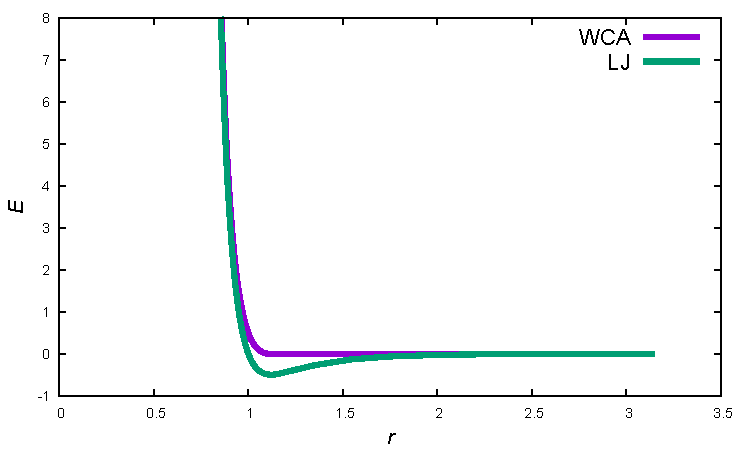
\includegraphics[width=15cm]{fig/dis-poen.pdf}
    \end{center}
    \caption{WCAとLJの原子間距離-ポテンシャルエネルギー。
    WCAポテンシャルはLJポテンシャルにカットオフ距離$r=r_c$を設けることにより、$r>r_c$でポテンシャルエネルギーが0になっている。}
    \label{fig:dis-poen}
\end{figure}
図{\ref{fig:dis-poen}に示すように、WCAポテンシャルはLJポテンシャルにカットオフ距離$r=r_c$を設けることにより、
$r>r_c$でポテンシャルエネルギーが0になっている。


\subsection{WCAポテンシャル粒子系の相図}\label{method-subsec:WCA-phase}
相図とは、熱力学的な状態量と物質や系の関係を表したものであり、相図の作成は、物性物理の分野において非常に重要である\cite{gaussian-phase}。

以下の図\ref{fig:wca-phase-diagram}に式(\ref{eq:wca})に示したWCAポテンシャル粒子系の相図の概念図を示す。

\begin{figure}[htbp]
    \begin{center}
        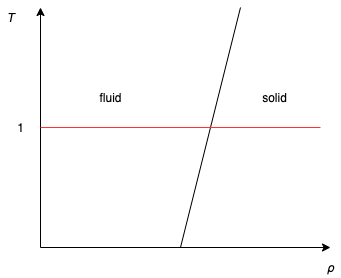
\includegraphics[width=12cm]{fig/wca-phase-diagram.png}
    \end{center}
    \caption{WCAポテンシャル粒子系の相図の概念図。
    数密度、温度とWCAポテンシャル粒子系の相の関係を示す。
    \ref{method-subsec:WCA-pressure}節では赤線上の状態点($T^*$=1.0)を観測する。}
    
    \label{fig:wca-phase-diagram}
\end{figure}

\newpage
図\ref{fig:wca-phase-diagram}に示すように、WCAポテンシャル粒子系はfluid(流体相)とsolid(固体相)の二相に分離する。
温度一定のまま密度を高くしていくと、ある密度で流体相から固体相への相転移を起こす。
この相転移近傍では、圧力の振る舞いが大きく変化するので、\ref{method-subsec:WCA-pressure}節では、
相転移近傍での圧力の振る舞いの変化を正しく捉えられるような手法を構築する。


\subsection{WCAポテンシャル粒子系における圧力測定}\label{method-subsec:WCA-pressure}
原子や分子の物理的な動きのコンピューターシミュレーション手法を分子動力学法(Molecular Dynamics method, MD)と言う\cite{molecular-dynamics}。
\ref{method-subsec:WCA-pressure}節では、式(\ref{eq:wca})に示したWCAポテンシャル粒子系における圧力の測定を分子動力学プログラムLarge-scale Atomic/Molecular Massively Parallel Simulator\,(LAMMPS)\cite{lammps}によるシミュレーションを用いて行う。
尚、本研究では、式(\ref{eq:wca})の${\sigma}$(原子直径の長さ)\,,\,${\varepsilon}$(ポテンシャルの深さ)を共に1.0とし、
図\ref{fig:wca-phase-diagram}で示した赤線上の状態点について、研究を進めるものとする。


本研究では、初期状態として1辺$L$、体積$V$の立方体の中に$N=2048$個の面心立方face-centered cubic\,(fcc)構造上に配置した分子を用意し、研究を進めるものとする。

\newpage
まず、以下の図\ref{fig:initial-state-molecule}に、初期状態の分子構造を示す。

\begin{figure}[htbp]
    \begin{center}
        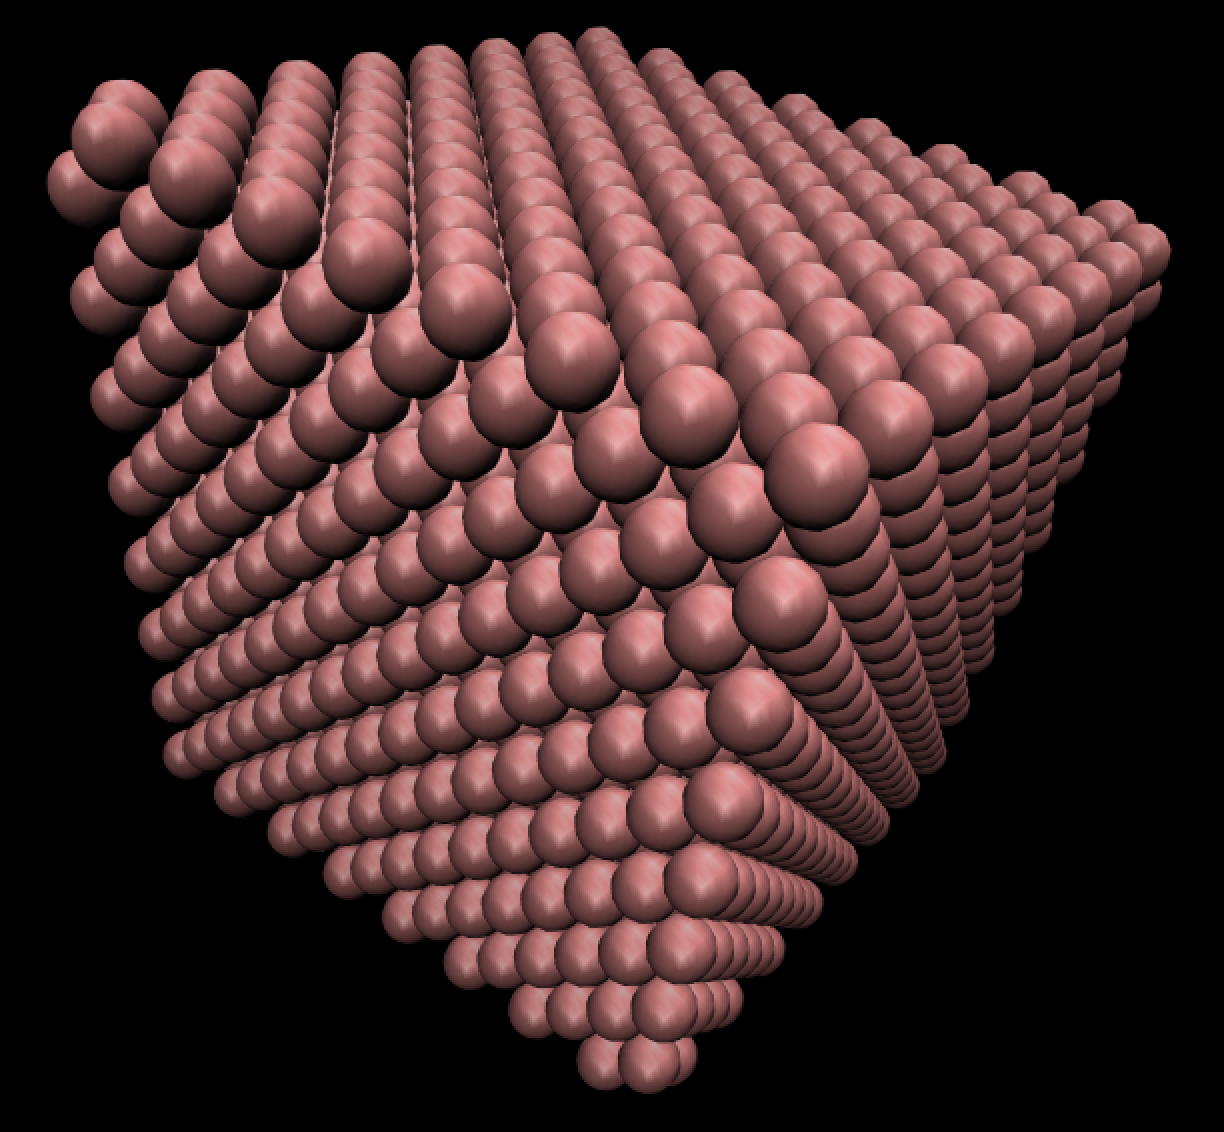
\includegraphics[width=12cm]{fig/initial-state-molecule.png}
    \end{center}
    \caption{初期状態の分子構造。
    fcc構造上に配置されている。}
    \label{fig:initial-state-molecule}
\end{figure}

上図\ref{fig:initial-state-molecule}に示すように初期状態では、分子がfcc構造上に配置されている。

この系の数密度は、
\large
\begin{equation}
\rho = {\frac{N}{V}}{\label{eq:density}}
\end{equation}
\normalsize
と表される。

数密度$\rho=0.01$から15.0まで、0.01刻みで圧力$P$を測定した。圧力の測定にはLAMMPSを用いた。
この初期条件のもと、タイムステップ0.001で20000実行のシミュレーションを行った。
尚、本研究ではNVTアンサンブルによりシミュレーション中の粒子数$N$、体積$V$、温度$T$が一定であることを前提とし、
温度は、$T=1.0$で制御できていたものとする。

二体相互作用をする粒子系における圧力は、ビリアル定理によって

\large
\begin{equation}
PV=NkT+{\frac{1}{3}}\langle\sum_{i=j}^N\vec{q_{ij}} \cdot \vec{r_{ij}}\rangle{\label{eq:Theoritical-pressure}}
\end{equation}
\normalsize
と表される\cite{Theoritical-pressure,virial-therom}。
ここで、$P$は圧力、$V$は体積、$N$は原子数、$k$はボルツマン定数、$T$は温度、$\vec{q_{ij}}$は粒子iと粒子jの相対位置ベクトル、$\vec{r_{ij}}$は原子間に働く力ベクトルである。

\ref{method-subsec:WCA-phase}節に示したように、WCAポテンシャル粒子系はある密度で流体ー固体相転移を起こすことから、
相転移点近傍で圧力の振る舞いが急激に変化すると考えられる。
\ref{results-sec:WCA-press}節では、MDシミュレーションで測定されたWCAポテンシャル粒子系における圧力の振る舞いを、
原子間の相互作用をほぼ無視できる低密度状態、流体相から固体相への相転移近傍の中密度状態、原子間の相互作用の寄与が大きい高密度状態において調べる。

\section{WCAポテンシャル粒子系における状態方程式の推定}\label{method-sec:WCA-equation}
\ref{method-sec:WCA-equation}節では、WCAポテンシャル粒子系における状態方程式の推定を行う。
\ref{method-subsec:virial}節、\ref{method-subsec:BWR}節では、圧力を密度に関する項で展開するビリアル展開、Benedict-Webb-Rubin\,(BWR)方程式、modified-Benedict–Webb–Rubin\,(mBWR)方程式の説明を示し、
\ref{method-subsec:WCA-equation}節では、\ref{results-sec:WCA-press}節で得た圧力$P$と数密度$\rho$の関係からWCAポテンシャル粒子系における状態方程式の推定を行う具体的な手法を示す。

\subsection{ビリアル展開}\label{method-subsec:virial}
気体の振る舞いを表す有望な記述の一つにビリアル展開と呼ぶものが存在する。
これは、Heikeによって1901年に提唱されたもの\cite{virial-Heike}で、多くの研究で利用されている\cite{virial-expansion-example1,virial-expansion-example2,virial-expansion-example3}。

理想気体の状態方程式は、

\large
\begin{equation}
P=RT{\rho}' \label{eq:ideal-gas-virial}
\end{equation}
\normalsize
と表されるが、
実存気体の状態方程式のビリアル展開は、式(\ref{eq:ideal-gas-virial})にずれを補正する項を付け加えたもので、

\large
\begin{equation}
P=RT{\rho}'+b_2{{\rho}'}^2+b_3{{\rho}'}^3+b_4{{\rho}'}^4+\cdots \label{eq:virial}
\end{equation}
\normalsize
と表され、圧力$P$をモル密度${\rho}'$の冪級数を用いて表現する。
ここで、$T$は温度、$R$は気体定数である。
式(\ref{eq:virial})のモル密度${\rho}'$のn番目の累乗の係数を第nビリアル係数と呼ぶ\cite{virial-expansion}。
これらのビリアル係数は、増加する原子数で構成される集団群における原子の相互作用を表し、第2、第3、第4のビリアル係数は、2つ、3つ、4つ...の分子を含む衝突が気体中で重要になったときの理想的な振る舞いからの逸脱を表す。
高密度になるほど、多体の相互作用の寄与が大きくなるので、圧力が高くなるにつれて、考慮されなければならないビリアル項が増加する\cite{virial-Heike}。

\subsection{Benedict-Webb-Rubin(BWR)方程式}\label{method-subsec:BWR}
\ref{method-subsec:virial}節のように、Heikeが提唱したビリアル展開は、圧力を密度の冪級数を用いて表現したものであるが、この式に経験則的に指数の項を付け加えたものをBenedict-Webb-Rubin(BWR)方程式と呼ぶ。
BWR方程式は、軽質炭化水素の熱力学的性質を予測するために、1940年にManson、George、Rubinによって提唱された\cite{BWR-equation:original}。
BWR方程式の原式は、圧力$P$をモル密度${\rho}'$と絶対温度$T$の関数として表現したもので、

\large
\begin{equation}
P=RT{\rho}'+\left(B_0RT-A_0-{\frac{C_0}{T^2}}\right){{\rho}'}^2+(bRT-a){{\rho}'}^3+{\frac{c}{T^2}}(1+{\gamma}{{\rho}'}^2)e^{-{\gamma}{{\rho}'}^2}{{\rho}'}^3+a{\alpha}{{\rho}'}^6\label{eq:BWR}
\end{equation}
\normalsize
と表される。

BWR方程式は、気体の状態方程式を表すことに概ね成功していたが、厳密には純粋な物質や混合物の熱力学的性質を予測するのに十分とは言えなかった。
そこで、1973年には、JacobsenとStewartによってBWR方程式の指数項をさらに増やした

\large
\begin{equation}
P=\sum_{n=1}^9a_n{{\rho}'}^n+\exp(-{\gamma}{{\rho}'}^2)\sum_{n=10}^{15}a_n{{\rho}'}^{2n-17}\label{eq:mBWR}
\end{equation}
\normalsize
と表されるmodified-Benedict–Webb–Rubin\,(mBWR)方程式が提唱\cite{m-BWR-equation}されたが、
依然として気体の状態方程式を完璧に再現することは出来なかった。
その後も、多くの研究者が気体の状態方程式の項を増やすことで、完璧な再現を試みた\cite{MCCARTY1974276,BWR-equation:13,BWR-equation:25}が、項の個数は際限なく増え、項自体の物理的意味も不明瞭であった。

\subsection{WCAポテンシャル粒子系における状態方程式の推定}\label{method-subsec:WCA-equation}
\ref{method-subsec:virial}節、\ref{method-subsec:BWR}節のように気体の状態方程式を項を増やすことによって再現しようと試みたが、項の個数は際限なく増え続けた。
また、BWR方程式に含まれる指数項は経験的に付け加えられたものであり、物理的な意味が不明瞭である。

そこで、機械学習により、より多くの候補からWCAポテンシャル粒子系における状態方程式を推定する方が効果的であると言える。
最終的には、機械学習が推定してきた項の物理的意味を考察することが目標であるが、
まず本研究では\ref{results-sec:WCA-press}節で示したWCAポテンシャル粒子系における圧力と数密度の関係に上記で示した最小二乗法を適用し、
圧力を数密度に関する低次の多項式で近似することにより、WCAポテンシャル粒子系における状態方程式を推定する。

以下、最小二乗法の説明を簡潔に示す。
今、想定される多項式を

\large
\begin{eqnarray}
f(x)=\sum_{j=0}^m a_jx^j \nonumber
\end{eqnarray}
\normalsize
で表すとし、
測定で得られた、$x_i$\,,\,$y_i$の組を
\large
\begin{eqnarray}
\{(x_1,y_1)\,,\,(x_2,y_2)\,,\,\cdots\,,\,(x_n,y_n)) \}\nonumber
\end{eqnarray}
\normalsize
とすると、残差の二乗和$S$は、

\large
\begin{eqnarray}
S=\sum_{i=1}^n (y_i-f(x_i))^2\label{eq:residual-error}
\end{eqnarray}
\normalsize
と表され、これを最小にする$f(x)$を求めることで最小二乗法は実現される。


式(\ref{eq:residual-error})を行列表示にすると、

\footnotesize
\begin{eqnarray}
S = \left(
        \left[
            \begin{array}{c}
            y_1\\
            y_2\\
            \vdots\\
            y_n
            \end{array}
        \right]
        -
        \left[
            \begin{array}{cccc}
            x_1^m & x_1^{m-1} & \cdots & x_1^0 \\
            x_2^m & x_2^{m-1} & \cdots & x_2^0 \\
            \vdots & \vdots & \vdots & \vdots\\
            x_n^m & x_n^{m-1} & \cdots & x_n^0 \\
            \end{array}
        \right]
        \left[
            \begin{array}{c}
            a_m\\
            a_{m-1}\\
            \vdots\\
            a_0
            \end{array}
        \right]
    \right)^T
    \left(
        \left[
            \begin{array}{c}
            y_1\\
            y_2\\
            \vdots\\
            y_n
            \end{array}
        \right]
        -
        \left[
            \begin{array}{cccc}
            x_1^m & x_1^{m-1} & \cdots & x_1^0 \\
            x_2^m & x_2^{m-1} & \cdots & x_2^0 \\
            \vdots & \vdots & \vdots & \vdots\\
            x_n^m & x_n^{m-1} & \cdots & x_n^0 \\
            \end{array}
        \right]
        \left[
            \begin{array}{c}
            a_m\\
            a_{m-1}\\
            \vdots\\
            a_0
            \end{array}
        \right]
  \right)\nonumber
\end{eqnarray}
\normalsize
と表される。
ここで、
\large
\begin{eqnarray}
Y=  \left[
        \begin{array}{c}
        y_1\\
        y_2\\
        \vdots\\
        y_n
        \end{array}
    \right]\,,\,
X=  \left[
        \begin{array}{cccc}
        x_1^m & x_1^{m-1} & \cdots & x_1^0 \\
        x_2^m & x_2^{m-1} & \cdots & x_2^0 \\
        \vdots & \vdots & \vdots & \vdots\\
        x_n^m & x_n^{m-1} & \cdots & x_n^0 \\
        \end{array}
    \right]\,,\,
A=  \left[
        \begin{array}{c}
        a_m\\
        a_{m-1}\\
        \vdots\\
        a_0
        \end{array}
    \right] \nonumber
\end{eqnarray}
\normalsize
とすると、

\large
\begin{eqnarray}
S &=& (Y-XA)^T(Y-XA)\nonumber\\
  &=& Y^TY-2A^TX^TY+A^TX^TXA\label{eq:queue-residual-error}
\end{eqnarray}
\normalsize
と表され、$S$を最小化する$A$を求める最小二乗問題に帰着する。
最小二乗問題は

\large
\begin{eqnarray}
    {\nabla}S=\frac{\partial S}{\partial A}
    =
    \left[
        \begin{array}{c}
            \frac{\partial S}{\partial a_m}\\
            \frac{\partial S}{\partial a_{m-1}}\\
            \vdots\\
            \frac{\partial S}{\partial a_0}
        \end{array}
    \right]
    =
    \left[
        \begin{array}{c}
            0\\
            0\\
            \vdots\\
            0
        \end{array}
    \right]\label{eq:Least-squares-problem}
\end{eqnarray}
\normalsize
から得られる連立方程式を$A$について解くことで表され、式(\ref{eq:queue-residual-error})\,,\,式(\ref{eq:Least-squares-problem})より、

\large
\begin{eqnarray}
    {\nabla}S&=&-2X^TY+2X^TXA=0\nonumber\\
    &{\Leftrightarrow}&{\ }{\ }X^TXA=X^TY\nonumber\\
    &{\Leftrightarrow}&{\ }{\ }A=(X^TX)^{-1}X^TY\label{eq:normal-equation}
\end{eqnarray}
\normalsize
で与えられる$A$を求めることで最小二乗法は完結する\cite{least-squares}。

\ref{results-sec:WCA-equation}節では、上記で述べたように\ref{results-sec:WCA-press}節で示したWCAポテンシャル粒子系における圧力と数密度の関係に
上記で示した最小二乗法を適用し、圧力を数密度に関する低次の多項式で近似することにより、WCAポテンシャル粒子系の状態方程式を推定する。
その後、推定したWCAポテンシャル粒子系における状態方程式の展開係数が先行研究と矛盾しないことを確認する。


\section{ガウス過程回帰によるWCAポテンシャル粒子系における効率的な状態方程式推定及び相図作成}\label{method-sec:Gauss}
\ref{method-sec:Gauss}節では、WCAポテンシャル粒子系における状態方程式を効率的に推定しつつ、相図を効率的に作成する。
\ref{method-subsec:Gauss}節では、ガウス過程回帰の説明を示し、
\ref{method-subsec:Gaussian-estimation}節では、\ref{results-sec:WCA-press}節で得た圧力$P$と数密度$\rho$の関係にガウス過程回帰を適用し、
WCAポテンシャル粒子系における状態方程式を効率的に推定しつつ、相図を効率的に作成する具体的な手法を示す。


\subsection{ガウス過程回帰}\label{method-subsec:Gauss}
ガウス過程回帰は、出力の不確実性も定量化できる確率的な補間予測を提供する\cite{machine-learning}。


$N$個の観測値、すなわち入力$x$\,,\,$y$の$N$個のペア

\large
\[
    \mathcal{D}=\{(x_1,y_1)\,,\,(x_2,y_2)\,,\,\cdots\,,\,(x_N,y_N)\}
\]
\normalsize
が与えられているとし、$\bm{X}=(x_1,\cdots,x_N)$\,,\,$\bm{y}=(y_1,\cdots,y_N)$とする。
簡単のため、$y$は平均が$\bm{0}$となるように正規化してあるとし、$y=f(x)$という関数$f$が平均$\bm{0}$のガウス過程

\large
\begin{eqnarray}
    f\,{\sim}\,GP(\bm{0},k(x,x'))\nonumber
\end{eqnarray}
\normalsize
から生成されているとする。
尚、$k(x,x')$は、カーネル関数と呼ばれるもので入力$x$の間の類似度を測るために使われるものであり\cite{Gauss-machine-learning}、測定値間の入力$x\,,\,x'$から求められる。

ここで、
\large
\begin{eqnarray}
\bm{y}=  
    \left[
        \begin{array}{c}
        y_1\\
        y_2\\
        \vdots\\
        y_N
        \end{array}
    \right] \nonumber
\end{eqnarray}
\normalsize
とおけば、この$\bm{y}$はガウス分布に従い、入力のすべてのペア$(x_n,x_{n'})$についてカーネル関数
$k(x,x')$を用いて、

\large
\begin{eqnarray}
K_{nn'}
=   k(x_n,x_{n'})\nonumber
\end{eqnarray}
\normalsize
で与えられるカーネル行列$\bm{K}$を使って、

\large
\begin{eqnarray}
\bm{y}
\,{\sim}\,{\mathcal{N}}(\bm{0},\bm{K})  \nonumber
\end{eqnarray}
\normalsize
が成立する。

今、データに含まれない$\bm{X}^*=(x_1^*,\cdots,x_M^*)$での$\bm{y}^*=(y_1^*,\cdots,y_M^*)$の値を予測する。
$\bm{y}$に$\bm{y}^*$を含めたものを新しく

\large
\begin{eqnarray}
\bm{y'}=  
    \left[
        \begin{array}{c}
        y_1\\
        y_2\\
        \vdots\\
        y_N\\
        y_1^*\\
        y_2^*\\
        \vdots\\
        y_M^*\\
        \end{array}
    \right] \nonumber
\end{eqnarray}
\normalsize
とし、$\bm{X}$および、$\bm{X}^*$から計算される$(N+M)×(N+M)$次元のカーネル行列を$\bm{K'}$とすると、
これら全体がまたガウス分布に従うので、

\large
\begin{eqnarray}
\bm{y'}
\,{\sim}\,{\mathcal{N}}(\bm{0},\bm{K'})  \nonumber
\end{eqnarray}
\normalsize
が成立する。

つまり、ガウス過程回帰は、\cite{Gaussian-Processes-for-Machine-Learning}で開発された導出に従って、観測された$\bm{y}$と予測された$\bm{y}^*$の同時分布が

\large
\begin{eqnarray}
    \left[
        \begin{array}{l}
            \bm{y} \\
            \bm{y}^* 
        \end{array}
    \right]
    {\sim}\,{\mathcal{N}}
    \left(0,
        \left[
            \begin{array}{cc}
                \bm{K} & \bm{k}_*\\    
                \bm{k}_*^T & \bm{k}_{**}
            \end{array}
        \right]
    \right) \label{eq:Gaussian-distribution}
\end{eqnarray}
\normalsize
のようなガウス分布に従う。
尚、$\bm{K}$は測定値の入力$x$と$x'$から求められ、$\bm{k}_*$は測定値の入力$x$と測定されていない入力$x'^*$から求められ、
$\bm{k}_{**}$は測定されていない入力$x^*$と測定されていない入力$x'^*$から求められる。

このガウス過程の予測分布は、式(\ref{eq:Gaussian-distribution})から、

\large
\begin{eqnarray}
p(\bm{y}^*|\bm{x}^*,\mathcal{D})
={\mathcal{N}}(\bm{k}_*^T\bm{K}^{-1}\bm{y}\,,\,\bm{k}_{**}-\bm{k}_*^T\bm{K}^{-1}\bm{k}_*)  \label{eq:Gaussian-predicted-distribution}
\end{eqnarray}
\normalsize
と表わされる。
以上から、未知のデータは平均を$E$、分散を$\sigma^2$とすると

\large
\begin{eqnarray}
    E&=&\bm{k}_*^T\bm{K}^{-1}\bm{y}\\ \label{eq:Gaussian-predicted-average}
    \sigma^2&=&\bm{k}_{**}-\bm{k}_*^T\bm{K}^{-1}\bm{k}_* \label{eq:Gaussian-predicted-decentration}
\end{eqnarray}
\normalsize
を満たすようなガウス分布に従う\cite{Gauss-machine-learning}。

式(\ref{eq:Gaussian-predicted-distribution})に示すようなガウス分布に基づき、未知のデータを推定するが、
このガウス分布を元に次に評価する点を決定する必要が生じる。この際に、式(\ref{eq:Gaussian-predicted-decentration})の分散$\sigma^2$の関数として
「獲得関数」と呼ばれるものを使用する。
獲得関数とは関連分野から借りてきた試行状態の「情報性」を定量化する用語に過ぎない\cite{acquisition-function}。


\subsection{ガウス過程回帰によるWCAポテンシャル粒子系の状態方程式の効率的推定}\label{method-subsec:Gaussian-estimation}
\ref{method-subsec:Gauss}節に示したガウス過程回帰を用いて、本研究では、WCAポテンシャル粒子系における数密度$\rho$と圧力$P$の関係を効率的に推定する。

本研究では、カーネル関数として、\cite{Gauss-machine-learning}で導入されている

\large
\begin{eqnarray}
    k(x,x')=\theta_1\exp\left(-\frac{(x-x')^2}{\theta_2}\right)+\theta_3\delta(x,x')\\ \label{eq:Gauss-kernel}
    (\theta_1=1.0,\theta_2=0.4,\theta_3=0.1) \nonumber \\ 
    (x=x':\delta(x,x')=1) \nonumber \\
    (x\,{\neq}\,x':\delta(x,x')=0) \nonumber
\end{eqnarray}
\normalsize
を採用する。

\ref{results-sec:WCA-press}節に、数密度$\rho=\{0.00,0.01,0.02,\cdots,15.0\}$と圧力$P$の関係を示したが、全データのうち端点となる、
$\{(P,\rho)\}=\{(0.00,0.00)\,,\,(15.0,1.83×10^7)\}$の二点を初期の入力データとして、ガウス過程回帰を適用する。
式(\ref{eq:Gaussian-predicted-average})の平均$E$が入力データから予測される関数を、
式(\ref{eq:Gaussian-predicted-decentration})の分散$\sigma^2$が入力データから予測される関数の不確かさを示すものとする。
また、各数密度における分散の平方根を取った標準偏差$\sigma$の大きさを獲得関数とし、この関数を最大にする、すなわち不確かさが最大の数密度を次の試行点として選択する。
この不確かさが最大となる数密度におけるWCAポテンシャル粒子系の圧力をMDシミュレーションにより新たに測定し、入力データを更新し、再度ガウス過程回帰を行う。
本研究では、以上の工程を繰り返し行い、WCAポテンシャル粒子系における状態方程式、相図の効率的推定を行う。
上記に示したアルゴリズムの簡易図を以下の図\ref{fig:algorithm}に示す。

\begin{figure}[htbp]
    \begin{center}
        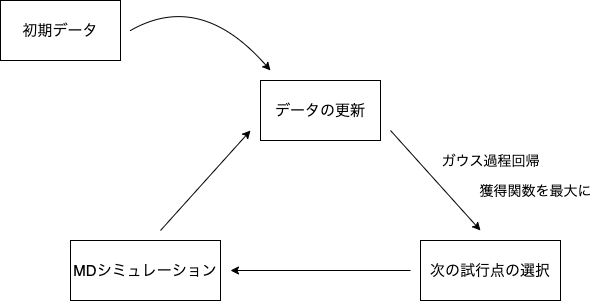
\includegraphics[width=15cm]{fig/algorithm.png}
    \end{center}
    \caption{本研究で用いるアルゴリズムの簡易図}
    \label{fig:algorithm}
\end{figure}

\chapter{結果} \label{chap:results}

\section{WCAポテンシャル粒子系における圧力測定}\label{results-sec:WCA-press}
\ref{results-sec:WCA-press}節では、各数密度においてMDシミュレーションで測定されたWCAポテンシャル粒子系における圧力の振る舞いを調べる。
まず、数密度$\rho$とMDシミュレーションで測定されたWCAポテンシャル粒子系における圧力$P$の関係を
以下の図\ref{fig:den-pre}に示す。

\begin{figure}[htbp]
    \begin{center}
        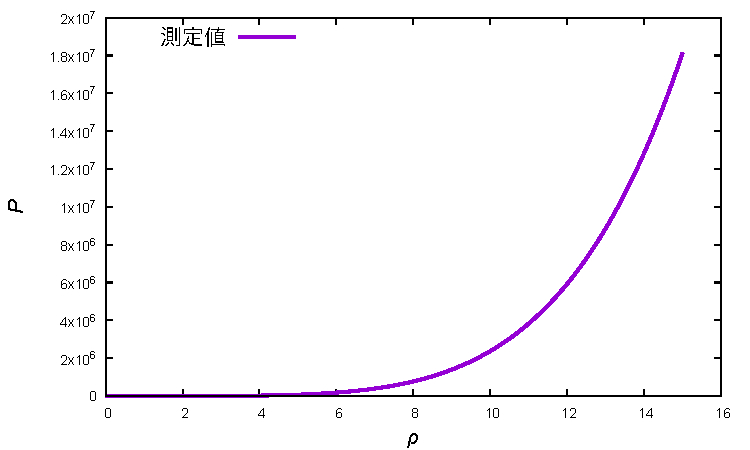
\includegraphics[width=15cm]{fig/den-pre.pdf}
    \end{center}
    \caption{WCAポテンシャル粒子系の圧力の測定値}
    \label{fig:den-pre}
\end{figure}

以下、\ref{results-subsec:WCA-press-low-density}節では原子間の相互作用をほぼ無視できる低密度状態、
\ref{results-subsec:WCA-press-middle-density}節では流体相から固体相への相転移近傍の中密度状態、
\ref{results-subsec:WCA-press-high-density}節では原子間の相互作用の寄与が大きい高密度状態において、
MDシミュレーションで測定されたWCAポテンシャル粒子系における圧力の振る舞いを抽出する。


\subsection{WCAポテンシャル粒子系における低密度状態の圧力}\label{results-subsec:WCA-press-low-density}
初期状態において、原子間の相互作用が作用する($原子間距離r=カットオフ距離r_c$)数密度は

\large
\begin{eqnarray}
\rho\,{\simeq}\,1.00 \nonumber
\end{eqnarray}
\normalsize
と表されるため、

\large
\begin{equation}
\rho\,{\leq}\,1.00 \label{eq:lowdensity-density}
\end{equation}
\normalsize
では、原子間の相互作用をほぼ無視できる。
上記の式(\ref{eq:lowdensity-density})を満たすような低密度状態における分子の状態の概念図を以下の図\ref{fig:lowdensity.png}に示す。

\begin{figure}[htbp]
    \begin{center}
        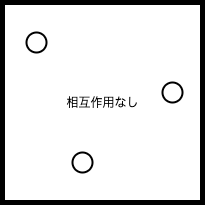
\includegraphics[width=7cm]{fig/lowdensity.png}
    \end{center}
    \caption{低密度状態における分子の状態の概念図。
    低密度状態では、分子間の相互作用はほぼ無視できる。}
    \label{fig:lowdensity.png}
\end{figure}

上図の図\ref{fig:lowdensity.png}のような低密度状態においては、原子間の相互作用をほとんど無視できるので、
圧力は式(\ref{eq:Theoritical-pressure})の第一項のみを用いて、
\large
\begin{equation}
PV\,{\simeq}\,NkT{\label{eq:ideal-gas}}
\end{equation}
\normalsize
と近似できる。


式(\ref{eq:ideal-gas})より、
\large
\begin{eqnarray}
PV\,&{\simeq}&\,NkT\nonumber\\
{\Leftrightarrow}{\ }{\ }P\,&{\simeq}&\,{\frac{N}{V}}kT\nonumber\\
{\Leftrightarrow}{\ }{\ }P\,&{\simeq}&\,{\rho}kT\nonumber
\end{eqnarray}
\normalsize
と書け、本研究では、$k=1$、$T=1$と設定し、MDシミュレーションにより圧力測定を行ったので、

\large
\begin{equation}
P\,{\simeq}\,{\rho} \label{eq:ideal-value}
\end{equation}
\normalsize
と表現できることが予測される。

式(\ref{eq:ideal-value})を「理論近似値」、本研究におけるMDシミュレーションにより測定された圧力を「測定値」とし、その結果を図\ref{fig:lowden_compare:den-pre}に示す。

\begin{figure}[htbp]
    \begin{center}
        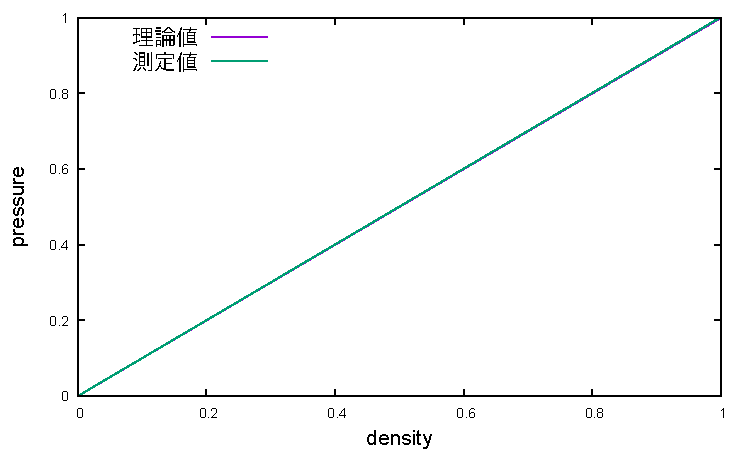
\includegraphics[width=15cm]{fig/lowden_compare:den-pre.pdf}
    \end{center}
    \caption{WCAポテンシャル粒子系における低密度状態の圧力の理論近似値と測定値の比較}
    \label{fig:lowden_compare:den-pre}
\end{figure}

図\ref{fig:lowden_compare:den-pre}から、低密度状態ではWCAポテンシャル粒子系の圧力は式(\ref{eq:ideal-gas})
と書けることがわかる。
これは、低密度状態では、「ほぼ」原子間の相互作用を無視でき、原子が理想気体のように振る舞うことに依存する。

\newpage
\subsection{WCAポテンシャル粒子系における中密度状態の圧力}\label{results-subsec:WCA-press-middle-density}
中密度状態では、相互作用がある分子ペアと持たない分子が存在する。
まず、中密度状態における分子の状態の概念図を以下の図\ref{fig:middledensity.png}に示す。

\begin{figure}[htbp]
    \begin{center}
        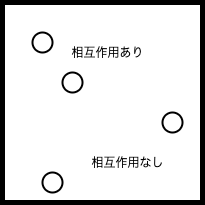
\includegraphics[width=7cm]{fig/middledensity.png}
    \end{center}
    \caption{中密度状態における分子の状態の概念図。
    中密度状態では、相互作用がある分子ペアと持たない分子が存在する}
    \label{fig:middledensity.png}
\end{figure}


流体相から固体相への相転移近傍の中密度状態では、相転移により圧力の振る舞いが急激に変化すると考えられる。
相転移近傍の中密度状態での数密度$\rho$とMDシミュレーションで測定されたWCAポテンシャル粒子系の圧力$P$の関係を
以下の図\ref{fig:middleden_den-pre}に示す。

\newpage
\begin{figure}[htbp]
    \begin{center}
        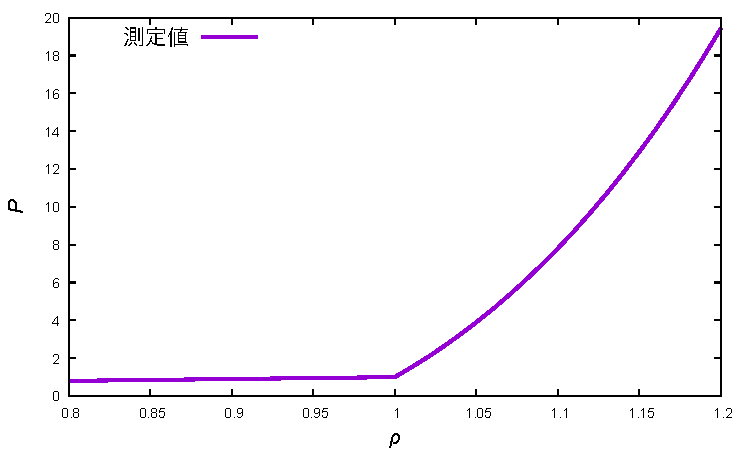
\includegraphics[width=15cm]{fig/middleden_den-pre.pdf}
    \end{center}
    \caption{WCAポテンシャル粒子系における中密度状態の数密度と圧力の関係。}
    \label{fig:middleden_den-pre}
\end{figure}


図\ref{fig:middleden_den-pre}から$\rho\,{\simeq}\,1$付近で相転移が起こり、圧力の振る舞いが急激に変化することを確認できた。
この相転移の存在により、圧力の振る舞いが急激に変化するので、WCAポテンシャル粒子系の状態方程式を\ref{method-subsec:virial}節で示したビリアル展開や、
\ref{method-subsec:BWR}節で示したBWR,m-BWR方程式を用いて表すと項の個数が際限なく増え、項自体の物理的意味も不明瞭になると考えられる。

\newpage
\subsection{WCAポテンシャル粒子系における高密度状態の圧力}\label{results-subsec:WCA-press-high-density}
高密度状態では、すべての分子ペアが相互作用を持つものと近似できる。
まず、高密度状態における分子の状態の概念図を以下の図\ref{fig:highdensity.png}に示す。

\begin{figure}[htbp]
    \begin{center}
        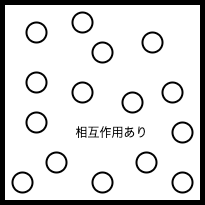
\includegraphics[width=7cm]{fig/highdensity.png}
    \end{center}
    \caption{高密度状態における分子の状態の概念図}
    \label{fig:highdensity.png}
\end{figure}


原子間の相互作用の寄与が大きい高密度状態では、圧力は式(\ref{eq:Theoritical-pressure})の第二項の影響を強く受ける。
高密度状態では、
密度が高くなればなるほど、式(\ref{eq:Theoritical-pressure})の第二項で考慮するものは、再隣接原子の寄与、第二隣接原子の寄与、第三隣接原子の寄与・・・と増えていく。

WCAポテンシャル粒子系において原子間に働く力$\vec{r_{ij}}$の大きさは、
WCAポテンシャル粒子系のポテンシャルエネルギーが式(\ref{eq:wca})に従うことから、

\large
\begin{eqnarray}
    | {\vec{r_{ij}}} |=\frac{d}{dr}\left(4\left(\left(\frac{1}{r}\right)^{12}-\left(\frac{1}{r}\right)^6\right)\right)=| 48r^{-13}-24r^{-7}| \nonumber
\end{eqnarray}
\normalsize
と書くことができるため、式(\ref{eq:Theoritical-pressure})の第二項の

\large
\begin{eqnarray}
    \sum_{i=j}^N\vec{q_{ij}} \cdot \vec{r_{ij}} \nonumber
\end{eqnarray}
\normalsize
は、距離に対して6乗で減衰することがわかる。

以上から、式(\ref{eq:Theoritical-pressure})の第二項への寄与はほとんどが再隣接原子であることから、本研究では、再隣接原子の寄与のみを考えるものとする。
第五隣接原子の寄与が生じる密度は、第五隣接原子間距離がWCAポテンシャル粒子系のカットオフ距離$r_c$と等しい、すなわち
$\rho\,{\simeq}\,14.7$と表される。
これより高密度の状態では、次々に原子間の相互作用が働いていくが、この高密度状態でも圧力が式(\ref{eq:Theoritical-pressure})において
再隣接原子の寄与のみを考慮したもので十分に表されることを確認する。

式(\ref{eq:ideal-value})において再隣接原子の寄与のみを考慮したものを「理論近似値」、本研究におけるMDシミュレーションにより測定された圧力を「測定値」とし、その結果を図\ref{fig:highden_compare:den-pre}に示す。

\begin{figure}[htbp]
    \begin{center}
        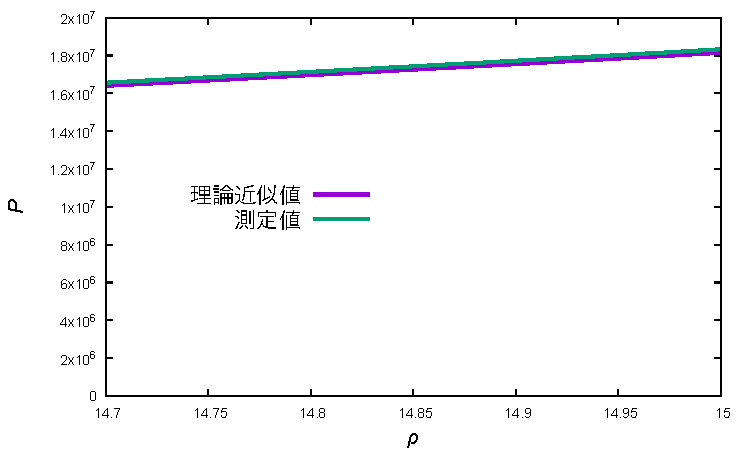
\includegraphics[width=15cm]{fig/highden_compare:den-pre.pdf}
    \end{center}
    \caption{WCAポテンシャル粒子系における高密度状態の圧力の理論近似値と測定値の比較}
    \label{fig:highden_compare:den-pre}
\end{figure}


図\ref{fig:highden_compare:den-pre}から、理論値と測定値のズレは1.2%以下であることがわかる。
このことから、第五隣接原子より離れた原子とも相互作用が働くほど高密度の状態でもWCAポテンシャル粒子系の圧力は式(\ref{eq:Theoritical-pressure})において
再隣接原子の寄与のみを考慮したもので十分に表されていることがわかる。

以上から、MDシミュレーションにより測定されたWCAポテンシャル粒子系の圧力の振る舞いを
原子間の相互作用をほぼ無視できる低密度状態、流体相から固体相への相転移近傍の中密度状態、原子間の相互作用の寄与が大きい高密度状態において確認できた。

\newpage
\section{WCAポテンシャル粒子系における状態方程式の推定}\label{results-sec:WCA-equation}
\ref{results-sec:WCA-press}節で示した圧力を数密度を含む項で展開することを試みたとき、\ref{method-subsec:virial}節で示したビリアル展開、
\ref{method-subsec:BWR}節で示したBWR,m-BWR方程式を用いると、\ref{results-subsec:WCA-press-middle-density}節で示した相転移の存在により、
項の個数が際限なく増え、項自体の物理的意味も不明瞭になると考えられる。
そこで、\ref{results-sec:WCA-equation}節では、\ref{results-sec:WCA-press}節で示したWCAパラメーター粒子系における圧力と数密度の関係に上記で示した最小二乗法を適用し、
圧力を数密度に関する低次の多項式で近似することにより、WCAポテンシャル粒子系の状態方程式を推定する。
尚、本研究における多項式近似とは、

\large
\begin{eqnarray}
    {{\rho}'}RT \nonumber &=& \frac{n}{V}RT \nonumber \\ 
    &=& \frac{N}{V}kT \nonumber \\ 
    &=& {\rho}kT \nonumber
\end{eqnarray}
\normalsize
を元に($k$:ボルツマン定数)、式(\ref{eq:virial})のビリアル展開を

\large
\begin{eqnarray}
    P=kT\rho+b_2\rho^2+b_3\rho^3+b_4\rho^4+\cdots\label{eq:search-virial} \nonumber
\end{eqnarray}
\normalsize
と表したものであるが、\ref{results-sec:WCA-press}節では、ボルツマン定数$k=1.0$、温度$T=1.0$としているので、
\large
\begin{equation}
    P=\rho+b_2\rho^2+b_3\rho^3+b_4\rho^4+\cdots\label{eq:modified-search-virial}
\end{equation}
\normalsize
と表される。

近似精度$A$を、各数密度$\rho$における圧力の測定値$P$と近似値$P'$の百分率誤差の絶対値の平均として定義すると、
近似精度は、

\large
\begin{equation}
    A=\frac{\sum_{i=1}^N\left(|\frac{P'-P}{P}\times100|\right)}{N}\,(%)\label{eq:percentage-error}
\end{equation}
\normalsize
と表される。
WCAポテンシャル粒子系の圧力を式(\ref{eq:modified-search-virial})のように数密度で2次〜5次に近似し、その近似精度を式(\ref{eq:percentage-error})に基づいて評価する。
この結果を以下の表\ref{table:approximation-accuracy}に示す。

\begin{table}[htbp]
    \begin{center}
        \caption{最小二乗法によるn次近似の近似精度}
            \begin{tabular}{c c}
               
                    n\,(次) & {\it{A}}\,(%) \\ \hline\hline
                    2 & 1.93E5 \\ 
                    3 & 2.32E5 \\ 
                    4 & 7.10E4\\ 
                    5 & 9.37\\ 
                    6 & 9.87 \\ 
                    7 & 19.77 \\ \hline
                
            \end{tabular}
    \end{center}
    \label{table:approximation-accuracy}
\end{table}

\newpage
低次から近似を行い、\ref{results-sec:WCA-press}節のMDシミュレーションにより測定されたWCAポテンシャル粒子系の圧力を数密度に関する多項式で近似することを試みたが、
上記の表\ref{table:approximation-accuracy}に基づくn次近似の近似精度から、本研究では、低次の多項式として5次の多項式を採用した。

最小二乗法により5次に近似されたWCAポテンシャル粒子系の状態方程式は、

\large
\begin{equation}
    P=\rho+8.40579\rho^2+-29.0885\rho^3+0.0158545\rho^4+24.2634\rho^5 \label{eq:5den-pre}
\end{equation}
\normalsize
と表された。
本研究で得られたMDシミュレーションによる圧力の値を「測定値」、式(\ref{eq:5den-pre})から得られる圧力の値を「5次近似値」とし、
以下の図\ref{fig:5den-pre}に示す。

\begin{figure}[htbp]
    \begin{center}
        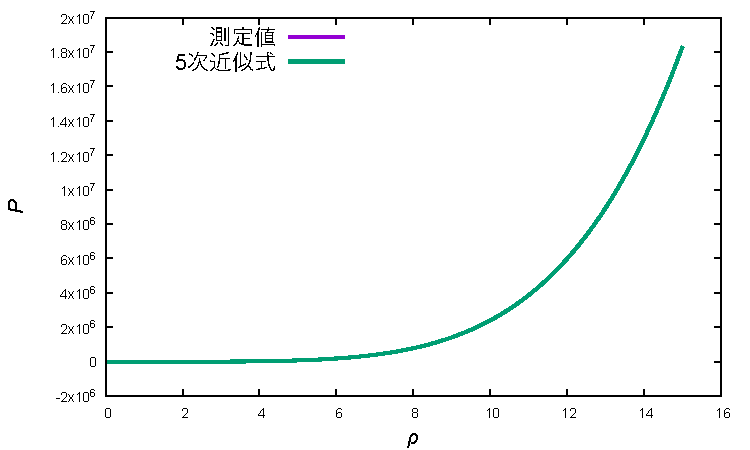
\includegraphics[width=14cm]{fig/5den-pre.pdf}
    \end{center}
    \caption{WCAポテンシャル粒子系におけるMDシミュレーションによる圧力の測定値と5次近似値の比較}
    \label{fig:5den-pre}
\end{figure}

\newpage
図\ref{fig:5den-pre}から、WCAポテンシャル粒子系の状態方程式は、式(\ref{eq:5den-pre})で書き表せているようではあるが、
表\ref{table:approximation-accuracy}から、近似精度としては十分と言えない。

続いて、式(\ref{eq:5den-pre})と推定されたWCAポテンシャルの状態方程式を先行研究と比較する。

\newpage
\section{ガウス過程回帰によるWCAポテンシャル粒子系における効率的な状態方程式推定及び相図作成}\label{results-sec:Gauss}
\ref{results-sec:Gauss}節では、\ref{results-sec:WCA-press}節で示した圧力$P$と数密度$\rho$の関係を効率的に推定する。

\ref{method-subsec:Gaussian-estimation}節に示したように、$\{(\rho,P)\}=\{(0.00,0.00)\,,\,(15.0,1.83×10^7)\}$の二点を初期の入力データとして、圧力$P$と数密度$\rho$の関係にガウス過程回帰を適用する。
以下の図\ref{fig:8plot}と\ref{fig:9plot}に本研究で採用したガウス過程回帰の推移の一部を示す。

\begin{figure}[htbp]
    \begin{minipage}{0.5\hsize}
    \begin{center}
     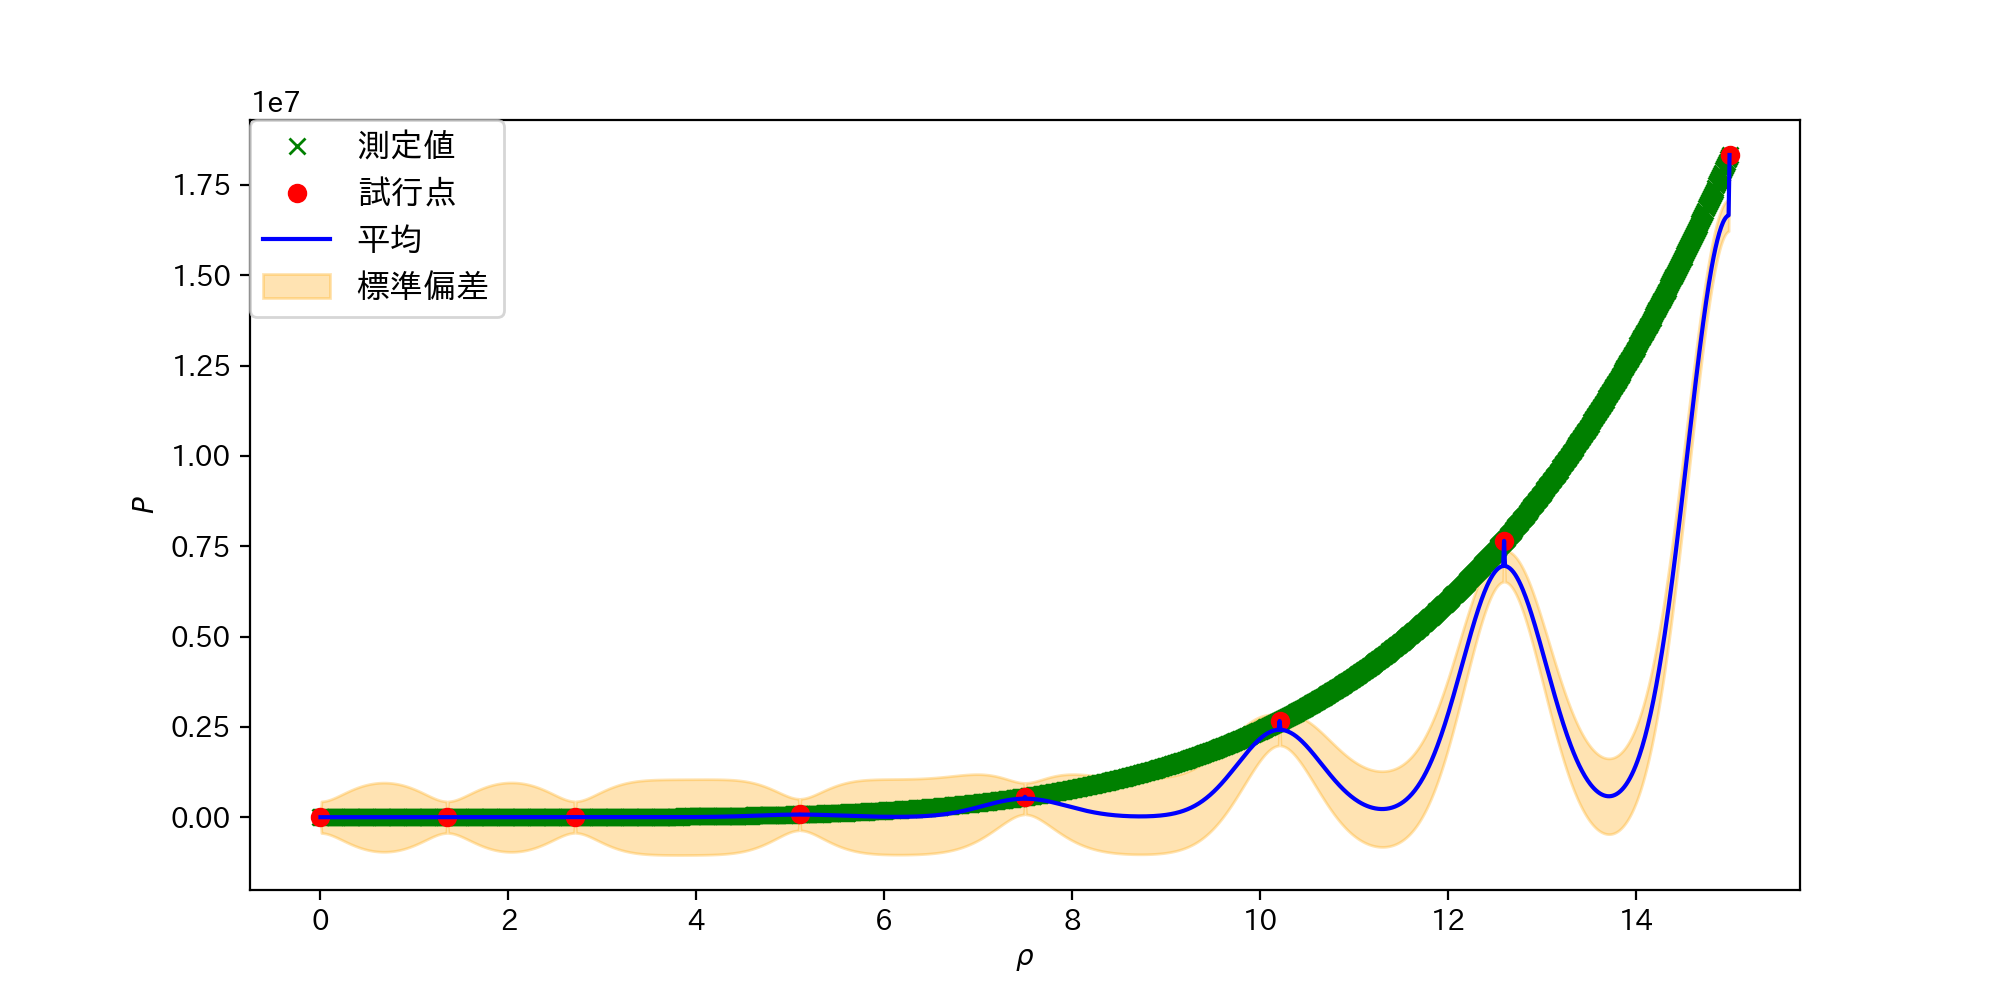
\includegraphics[width=75mm]{fig/8plot-Gauss.png}
     \caption{8点を入力とした時の平均と標準偏差}
     \label{fig:8plot}
    \end{center}
    \end{minipage}
    \begin{minipage}{0.5\hsize}
    \begin{center}
     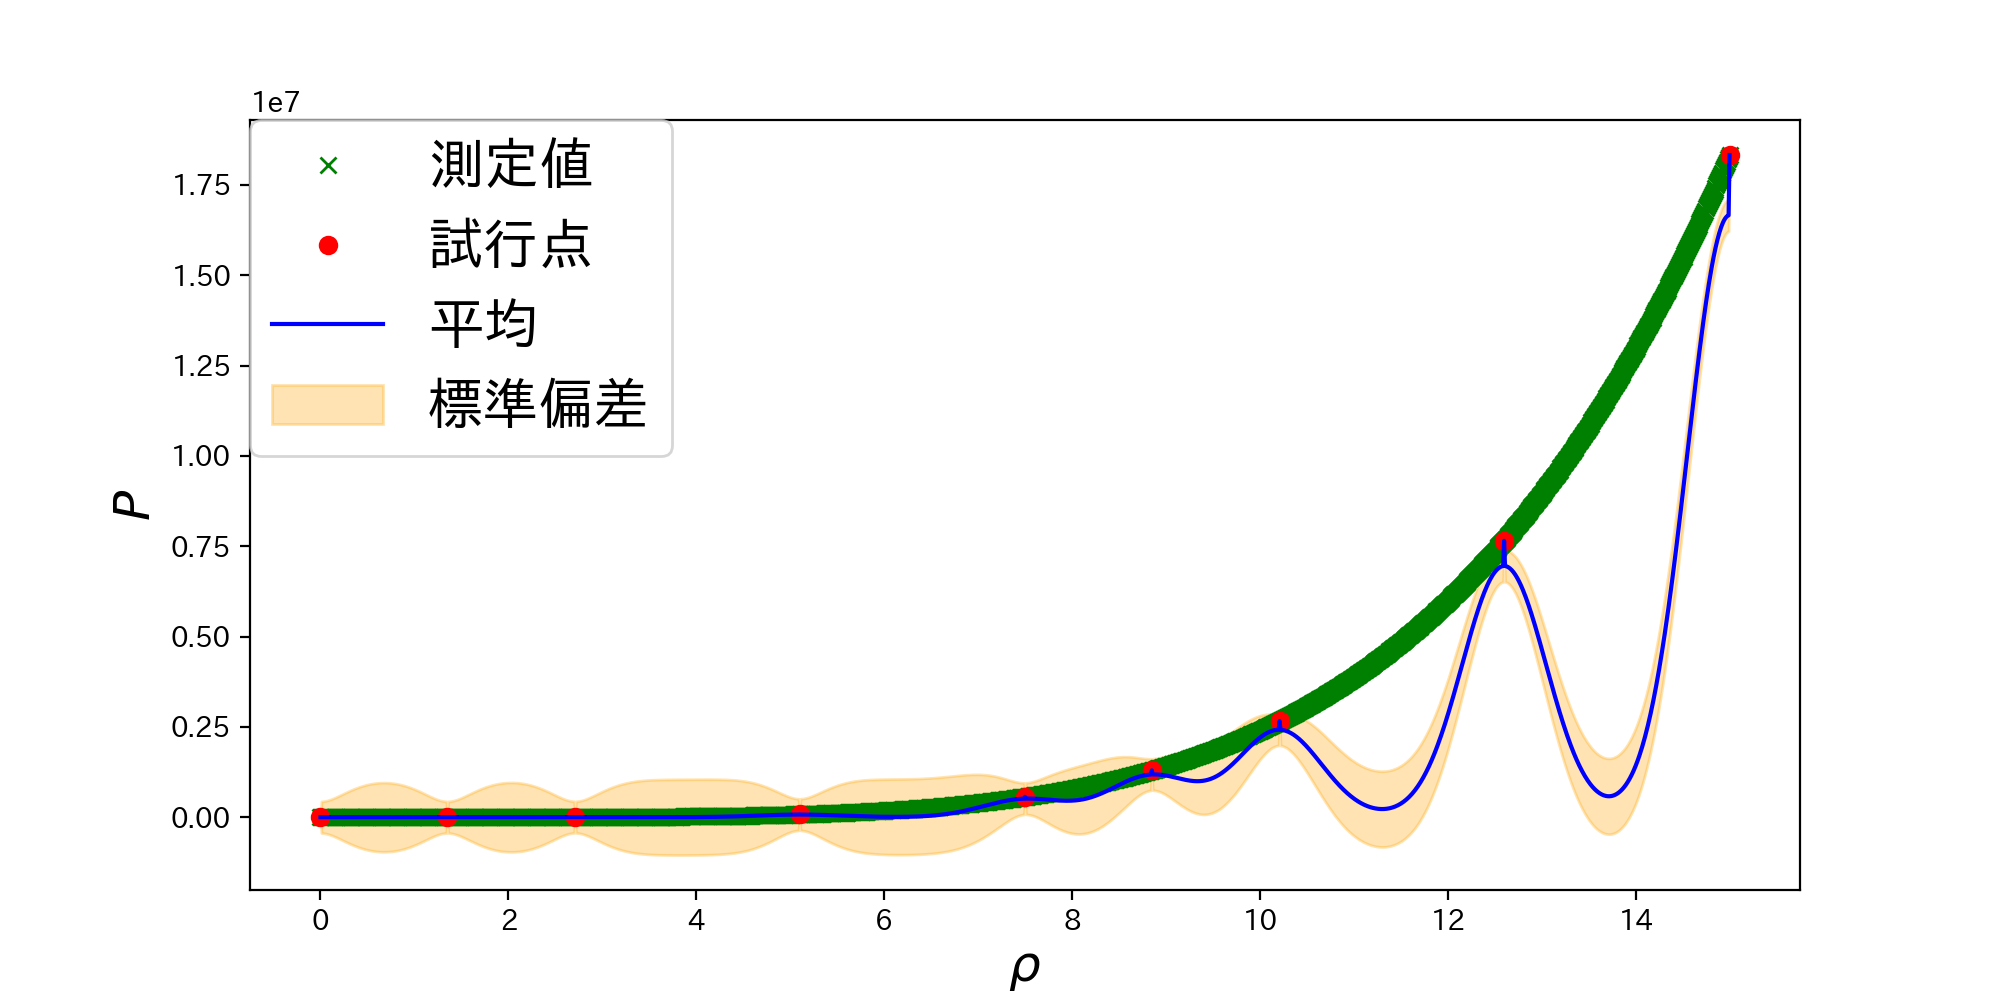
\includegraphics[width=75mm]{fig/9plot-Gauss.png}
     \caption{9点を入力とした時の平均と標準偏差}
     \label{fig:9plot}
    \end{center}
    \end{minipage}
   \end{figure}

上図\ref{fig:8plot}は、測定した8点を入力データとしてガウス過程回帰を適用し、平均と標準偏差を示したものである。
(尚、本研究では、標準偏差の可視化のために標準偏差を1000000倍に調整している)
\ref{method-subsec:Gaussian-estimation}節に示したように、図\ref{fig:8plot}において標準偏差(=不確かさ)の大きさが最大となる数密度${\rho}\simeq9$
の点を次の試行点として選択する。この数密度$\rho$における圧力$P$をMDシミュレーションにより求め、入力データに追加し、ガウス過程回帰を適用したものが図\ref{fig:9plot}である。
図\ref{fig:8plot}に比べ、\ref{fig:9plot}は標準偏差(=不確かさ)が小さくなっていることが確認できる。
このように、不確かさが最大となる点を選択し、ガウス過程回帰を適用することを繰り返すことで、効率的にプロットを行っていく。

上記のようなガウス過程回帰を行うことにより、26点を入力データとした時、\ref{results-sec:WCA-press}節で示した
圧力$P$と密度$\rho$の関係を再現することに成功した。
以下の図\ref{fig:26plot}にその様子を示す。

\begin{figure}[htbp]
    \begin{center}
        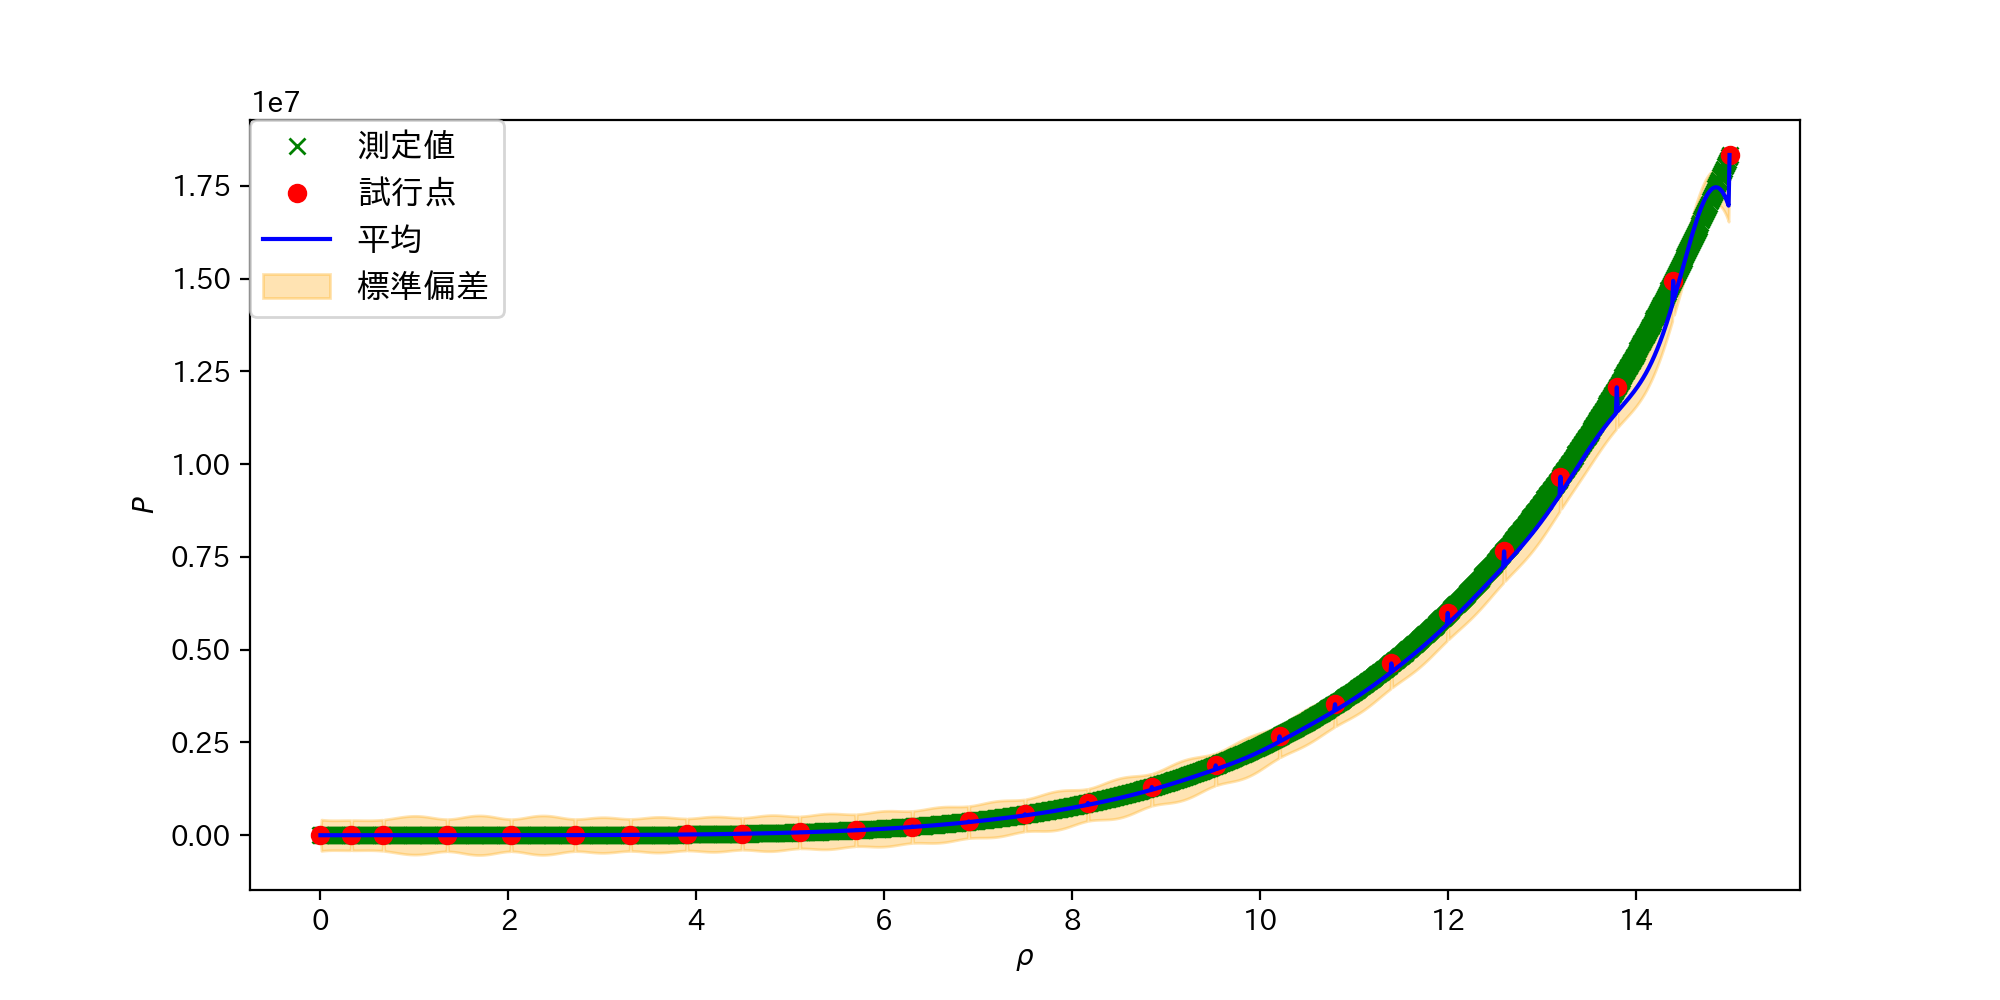
\includegraphics[width=15cm]{fig/26plot-Gauss.png}
    \end{center}
    \caption{26点を入力とした時の平均と標準偏差}
    \label{fig:26plot}
\end{figure}

\newpage
上図\ref{fig:26plot}から、26点の入力データで\ref{results-sec:WCA-press}節で示した
圧力$P$と密度$\rho$の関係を再現することに成功していることが読み取れる。

続いて、上図\ref{fig:26plot}に示した試行点を元に、WCAポテンシャル粒子系の状態方程式の推定が効率的に行うことが出来るかを調べる。
$\rho=0.00,0.60,1.20,\cdots,15.0$と$\rho=0.00〜15.0$に26点等間隔で用意したものとその圧力のペアを入力データ1、
図\ref{fig:26plot}に示した26点の試行点を入力データ2とする。
まず、以下に入力データ1と入力データ2における数密度$\rho$を示す。

\begin{table}[htbp]
    \begin{center}
        \caption{入力データ1,2における数密度$\rho$}
            \begin{tabular}{c||c c c c c c c c c c c c c c c c c c c c c c c c c c}
               
                    入力データ1& 0.00&0.60&1.20&1.80&2.40&3.00&3.60&4.20&4.80&5.40&6.00&6.60&7.20\\
                    &7.80&8.40&9.00&9.60&10.20&10.80&11.40&12.00&12.60&13.20&13.80&14.40&15.00\\ \hline
                    入力データ2& 0.00&0.33&0.67&1.35&2.03&2.71&3.30&3.90&4.49&5.10&5.70&6.30&6.90\\
                    &7.50&8.17&8.85&9.53&10.21&10.80&11.40&12.00&12.60&13.20&13.80&14.40&15.00
                    
            \end{tabular}
    \end{center}
    \label{table:compare-Gauss}
\end{table}
上記の表\ref{table:compare-Gauss}で示した各入力データにおける数密度$\rho$と圧力$P$に対して、\ref{results-sec:WCA-equation}節で採用した最小二乗法の5次式近似
を適用し、それそれの入力データに対する近似精度を式(\ref{eq:percentage-error})で評価する。
以下の表\ref{table:compare-approximation-accuracy}に、入力データ1と入力データ2に対する近似精度を示す。

\begin{table}[htbp]
    \begin{center}
        \caption{入力データ1,2に対する近似精度$A$}
            \begin{tabular}{c c}
                    入力データ1\,(%) & 入力データ2\,(%) \\ \hline\hline
                    9.191 & 9.139
            \end{tabular}
    \end{center}
    \label{table:compare-approximation-accuracy}
\end{table}
上記の表\ref{table:compare-approximation-accuracy}から、ガウス過程回帰を適用した入力データ2を元にした時、
数密度を等間隔にとった入力データ1よりもWCAポテンシャル粒子系の状態方程式を推定出来ていることがわかる。
以上から、\ref{method-subsec:Gaussian-estimation}節で提示したアルゴリズムにより、WCAポテンシャルの状態方程式を効率的に推定することに成功した。

最後に、上図\ref{fig:26plot}に示した試行点を元に、WCAポテンシャル粒子系の相図を効率的に作成することが出来るかを調べる。
WCAポテンシャルの相転移は、\ref{results-subsec:WCA-press-middle-density}節の図\ref{fig:middleden_den-pre}から、
数密度$\rho\,{\simeq}1.00$で起こる。そこで、WCAポテンシャル粒子系において効率的に相図を作成するために、ガウス過程回帰を用いて標準偏差(不確かさ)が最大の点を選択していくような\ref{method-subsec:Gaussian-estimation}節で提示したアルゴリズムにより、
相転移近傍の急激な圧力の変化を機械が捉えると予測したが、表\ref{table:compare-approximation-accuracy}より
相転移近傍である$\rho=1.00$付近を重点的に探索するようなアルゴリズムは構築出来ていない。
以上から、\ref{method-subsec:Gaussian-estimation}節で提示したアルゴリズムでは、WCAポテンシャルの相図を効率的に作成することに失敗した。

\chapter{考察および結論} \label{chap:summary}

考察は、「研究の背景」及び「目的」において提起した問題に正しく答えるようにする。得られた結果は満足すべきものだったか?不満があるならその理由はなにか?解決できそうなのか?また、「大きい理由」にも言及する。本研究によりどのような課題が見つかったかを書き、この分野における「研究の流れ」においてのような位置づけにあるかを説明した上で、今後、どのような発展の方向があるかについて書く。

本研究では、ガウス過程回帰を用いることにより、WCAポテンシャルにおける効率的な状態方程式の推定及び、相図作成を目的とした。

\chapter*{謝辞}

まず、私を研究室に迎えれていただき、研究を進める上で、基礎的な部分から複雑な部分まで多くの指導をしていただいた渡辺宙志准教授には大変感謝しております。
研究部分のみならず、私たちの様子を常に気にかけ、研究設備や生活面でのサポートもしていただきましたこと心より御礼申し上げます。

また、同じ研究室に所属していた藤田くん、四辻くん、佐藤くんは、同じ部屋で研究を進め、分からない部分をお互いに共有しながら共に切磋琢磨できたと思います。
研究の合間に、昼ごはんを食べにいったり、他愛もない話をしたりと、息抜きをしながら研究を進めることが出来ましたこと、深く感謝致します。

最後に、研究のみならず、学生生活を様々な面でサポートしてくださった両親に深く感謝致します。


\appendix

\chapter{ソースコード}

\lstinputlisting[caption = 適当なPythonスクリプト, label = prog:sample]{src/sample.py}

\bibliographystyle{junsrt}
\bibliography{reference}

\end{document}